\documentclass[11pt]{beamer}
%\documentclass[11pt,handout]{beamer}

\usepackage{multimedia}

%\usetheme[secheader]{Boadilla}
\usetheme{Boadilla}

%\setbeameroption{hide notes}
%\setbeameroption{show notes}
%\setbeameroption{show only notes}
%\setbeamertemplate{note page}[plain]

\usefonttheme{structuresmallcapsserif}
\setbeamerfont{frametitle}{size=\normalsize}
\setbeamertemplate{navigation symbols}{}

\AtBeginSection[]{}

\setbeamercovered{invisible}

% Custom packages
\usepackage{bibentry}
\usepackage{color}

\usepackage{animate}

% Customization
\newcommand{\footcite}[1]{$^[$\footnote{\begin{tiny}\bibentry{#1}\end{tiny}}$^]$}

\renewcommand{\emph}[1]{\textbf{#1}}

\newcommand{\taskparam}{{\color{red} \tau}}
\newcommand{\skillparam}{{\color{blue} \theta}}

\newcommand{\newblock}{}

% Author, Title, etc.
\title[EWRL 2013]{Learning Skill Templates for Parameterized Tasks}
\author[Metzen \& Fabisch]{Jan Hendrik Metzen and Alexander Fabisch}
\institute[University Bremen]{AG Robotik, University Bremen\\ Project BesMan \url{http://robotik.dfki-bremen.de/de/forschung/projekte/besman.html}}
\date[05-09/08/13]{EWRL, August 05-09, 2013}

\begin{document}

\frame{\titlepage
       \bibliographystyle{abbrv}
       \nobibliography{../references}}

\begin{frame}{Motivation: Learn Skills for Robotic Mobile Manipulation}
   \begin{center}
   \movie[width=8cm,height=6cm,externalviewer]
             {\includegraphics[width=8cm,height=6cm]{PA10_Throwing_Ball}}{targets_short.avi} \\
   Example: learn to throw a ball at different targets
   \end{center}
\end{frame}

\begin{frame}{Multi-Task Reinforcement Learning}
  Given:
  \begin{itemize}
    \item Class of RL problems parameterized by $\taskparam \in T \subseteq \mathbb{R}^n$
    \item Task distribution $P(\taskparam)$ {\tiny [in this talk uniform over $T$]}
    \item Skill represented by a parameterized policy with parameter vector $\skillparam \in
\mathbb{R}^m$
    \item Means for determining return $J(\skillparam, \taskparam)$ of the skill parametrized by $\skillparam$ in task $\taskparam$
  \end{itemize}
  \pause
  Parameterized skill \footcite{da_silva_learning_2012}:
  \begin{itemize}
    \item Learn a function $\hat{\Theta}: \taskparam \mapsto \skillparam_\taskparam$ from task vector $\taskparam$ to a skill vector $\skillparam_\taskparam$
    \item Objective: $\hat{\Theta}$ similar to $\Theta^* = \arg\max_\Theta \int P(\taskparam)J(\Theta(\taskparam),\taskparam)d\taskparam$
    \item Typically: $\hat{\Theta}(\taskparam) \neq \arg\max_\skillparam J(\skillparam,\taskparam)$
  \end{itemize}
  \pause
  Our approach: give more than point estimate $\hat{\Theta}(\taskparam)$
\end{frame}

\begin{frame}{Learning Skill Templates}
  Given:
  \begin{itemize}
    \item Training set from $K$ source tasks $E = \left\{(\taskparam_i, \skillparam_{\taskparam_i}) \vert i=1,\dots,K\right\}$ with $J(\skillparam_{\taskparam_i},\taskparam_i) \approx J(\skillparam_{\taskparam_i}^*,\taskparam_i)$
    \item $E$ can be generated using RL (e.g., direct policy search) in each of the tasks
  \end{itemize}
 \pause
 Skill Templates
 \begin{itemize}
    \item \emph{Goal}: Transfer procedural knowledge contained in $E$ to novel, $(K+1)$st tasks $\tau$
    \item \emph{Idea}: learn to initialize policy search for new task such that close-to-optimal policies can be learned more sample-efficiently
    \item Skill template: $\psi: \taskparam \mapsto \mathcal{N}(\Theta(\taskparam), \Omega(\taskparam))$
    \item Normal distribution over policy parameter space, where
    \begin{itemize}
      \item $\Theta(\taskparam) \in \mathbb{R}^m$ determines starting point for policy search
      \item $\Omega(\taskparam) \in \mathbb{R}^{m\times m}$ controls initial exploration
    \end{itemize}
    \item Skill template learned from $E$
  \end{itemize}

\end{frame}

\begin{frame}{Approach}
  \begin{itemize}
    \item Represent skills using dynamical systems movement primitives (DMPs)\footcite{Ijspeert2013}\footcite{mulling_learning_2012}
    \item Learn source task policies using policy search based on CMA-ES \footcite{hansen_completely_2001}
    \item Learn $\Theta: \taskparam \mapsto \skillparam_\taskparam$ from E using Gaussian Process Regression (GPR) \footcite{rasmussen_gaussian_2006}
    \item Restrict $\Omega$ to the diagonal case {\tiny [for now]}:
    \begin{enumerate}
      \item Weight-proportional exploration: $\Omega(\taskparam)_{ii}$ proportional to $\vert\Theta(\taskparam)_i\vert$
      \item Uncertainty exploration: $\Omega(\taskparam)_{ii}$ proportional to uncertainty in GPR's prediction of $\Theta_i$
    \end{enumerate}
    \item Normalize mean eigenvalue of $\Omega(\taskparam)$
  \end{itemize}
\end{frame}

\begin{frame}{Test domain}
  \begin{itemize}
    \item Learn to throw a ball with a simulated PA-$10$
    \item $\taskparam \in \mathbb{R}^2$: target position on floor
    \item $\skillparam \in \mathbb{R}^{96}$: DMP parameters controlling robot in joint space ($8$ joints):
    \begin{itemize}
      \item Joint's trajectory ($10$ parameters per joint)
      \item Joint's final position and velocity ($2$ parameters per joint)
    \end{itemize}
    \item $J(\skillparam,\taskparam)$: Negative of squared distance of thrown ball from target
  \end{itemize}
  \begin{center}
    \includegraphics[width=.6\linewidth]{PA10_Throwing_Ball}
  \end{center}
\end{frame}

\begin{frame}{Illustration: Ball Throwing (1/2)}
   \begin{center}
   Error of $\Theta(\taskparam)$ vs.\,Number of Source Tasks
   \end{center}
   \begin{center}
         \only<1>{\includegraphics[width=\linewidth]
                   {plots/prediction_error_00}}
         \only<2>{\includegraphics[width=\linewidth]
                   {plots/prediction_error_01}}
         \only<3>{\includegraphics[width=\linewidth]
                   {plots/prediction_error_03}}
         \only<4>{\includegraphics[width=\linewidth]
                   {plots/prediction_error_05}}
         \only<5>{\includegraphics[width=\linewidth]
                   {plots/prediction_error_09}}
   \end{center}
\end{frame}

\begin{frame}{Illustration: Ball Throwing (2/2)}
   \begin{center}
   Error during Learning (Tabula Rasa vs.\,Skill Template (Uncertainty))
   \end{center}
   \begin{center}
         \only<1>{\includegraphics[width=\linewidth]
                   {plots/error_during_learning_00}}
         \only<2>{\includegraphics[width=\linewidth]
                   {plots/error_during_learning_01}}
         \only<3>{\includegraphics[width=\linewidth]
                   {plots/error_during_learning_02}}
         \only<4>{\includegraphics[width=\linewidth]
                   {plots/error_during_learning_03}}
         \only<5>{\includegraphics[width=\linewidth]
                   {plots/error_during_learning_04}}
         \only<6>{\includegraphics[width=\linewidth]
                   {plots/error_during_learning_05}}
   \end{center}
\end{frame}

\begin{frame}{Results: Ball Throwing}
   \begin{center}
   Learning Curve (Tabula Rasa vs.\,ST with different $\Omega$)
   \end{center}
   \begin{center}
         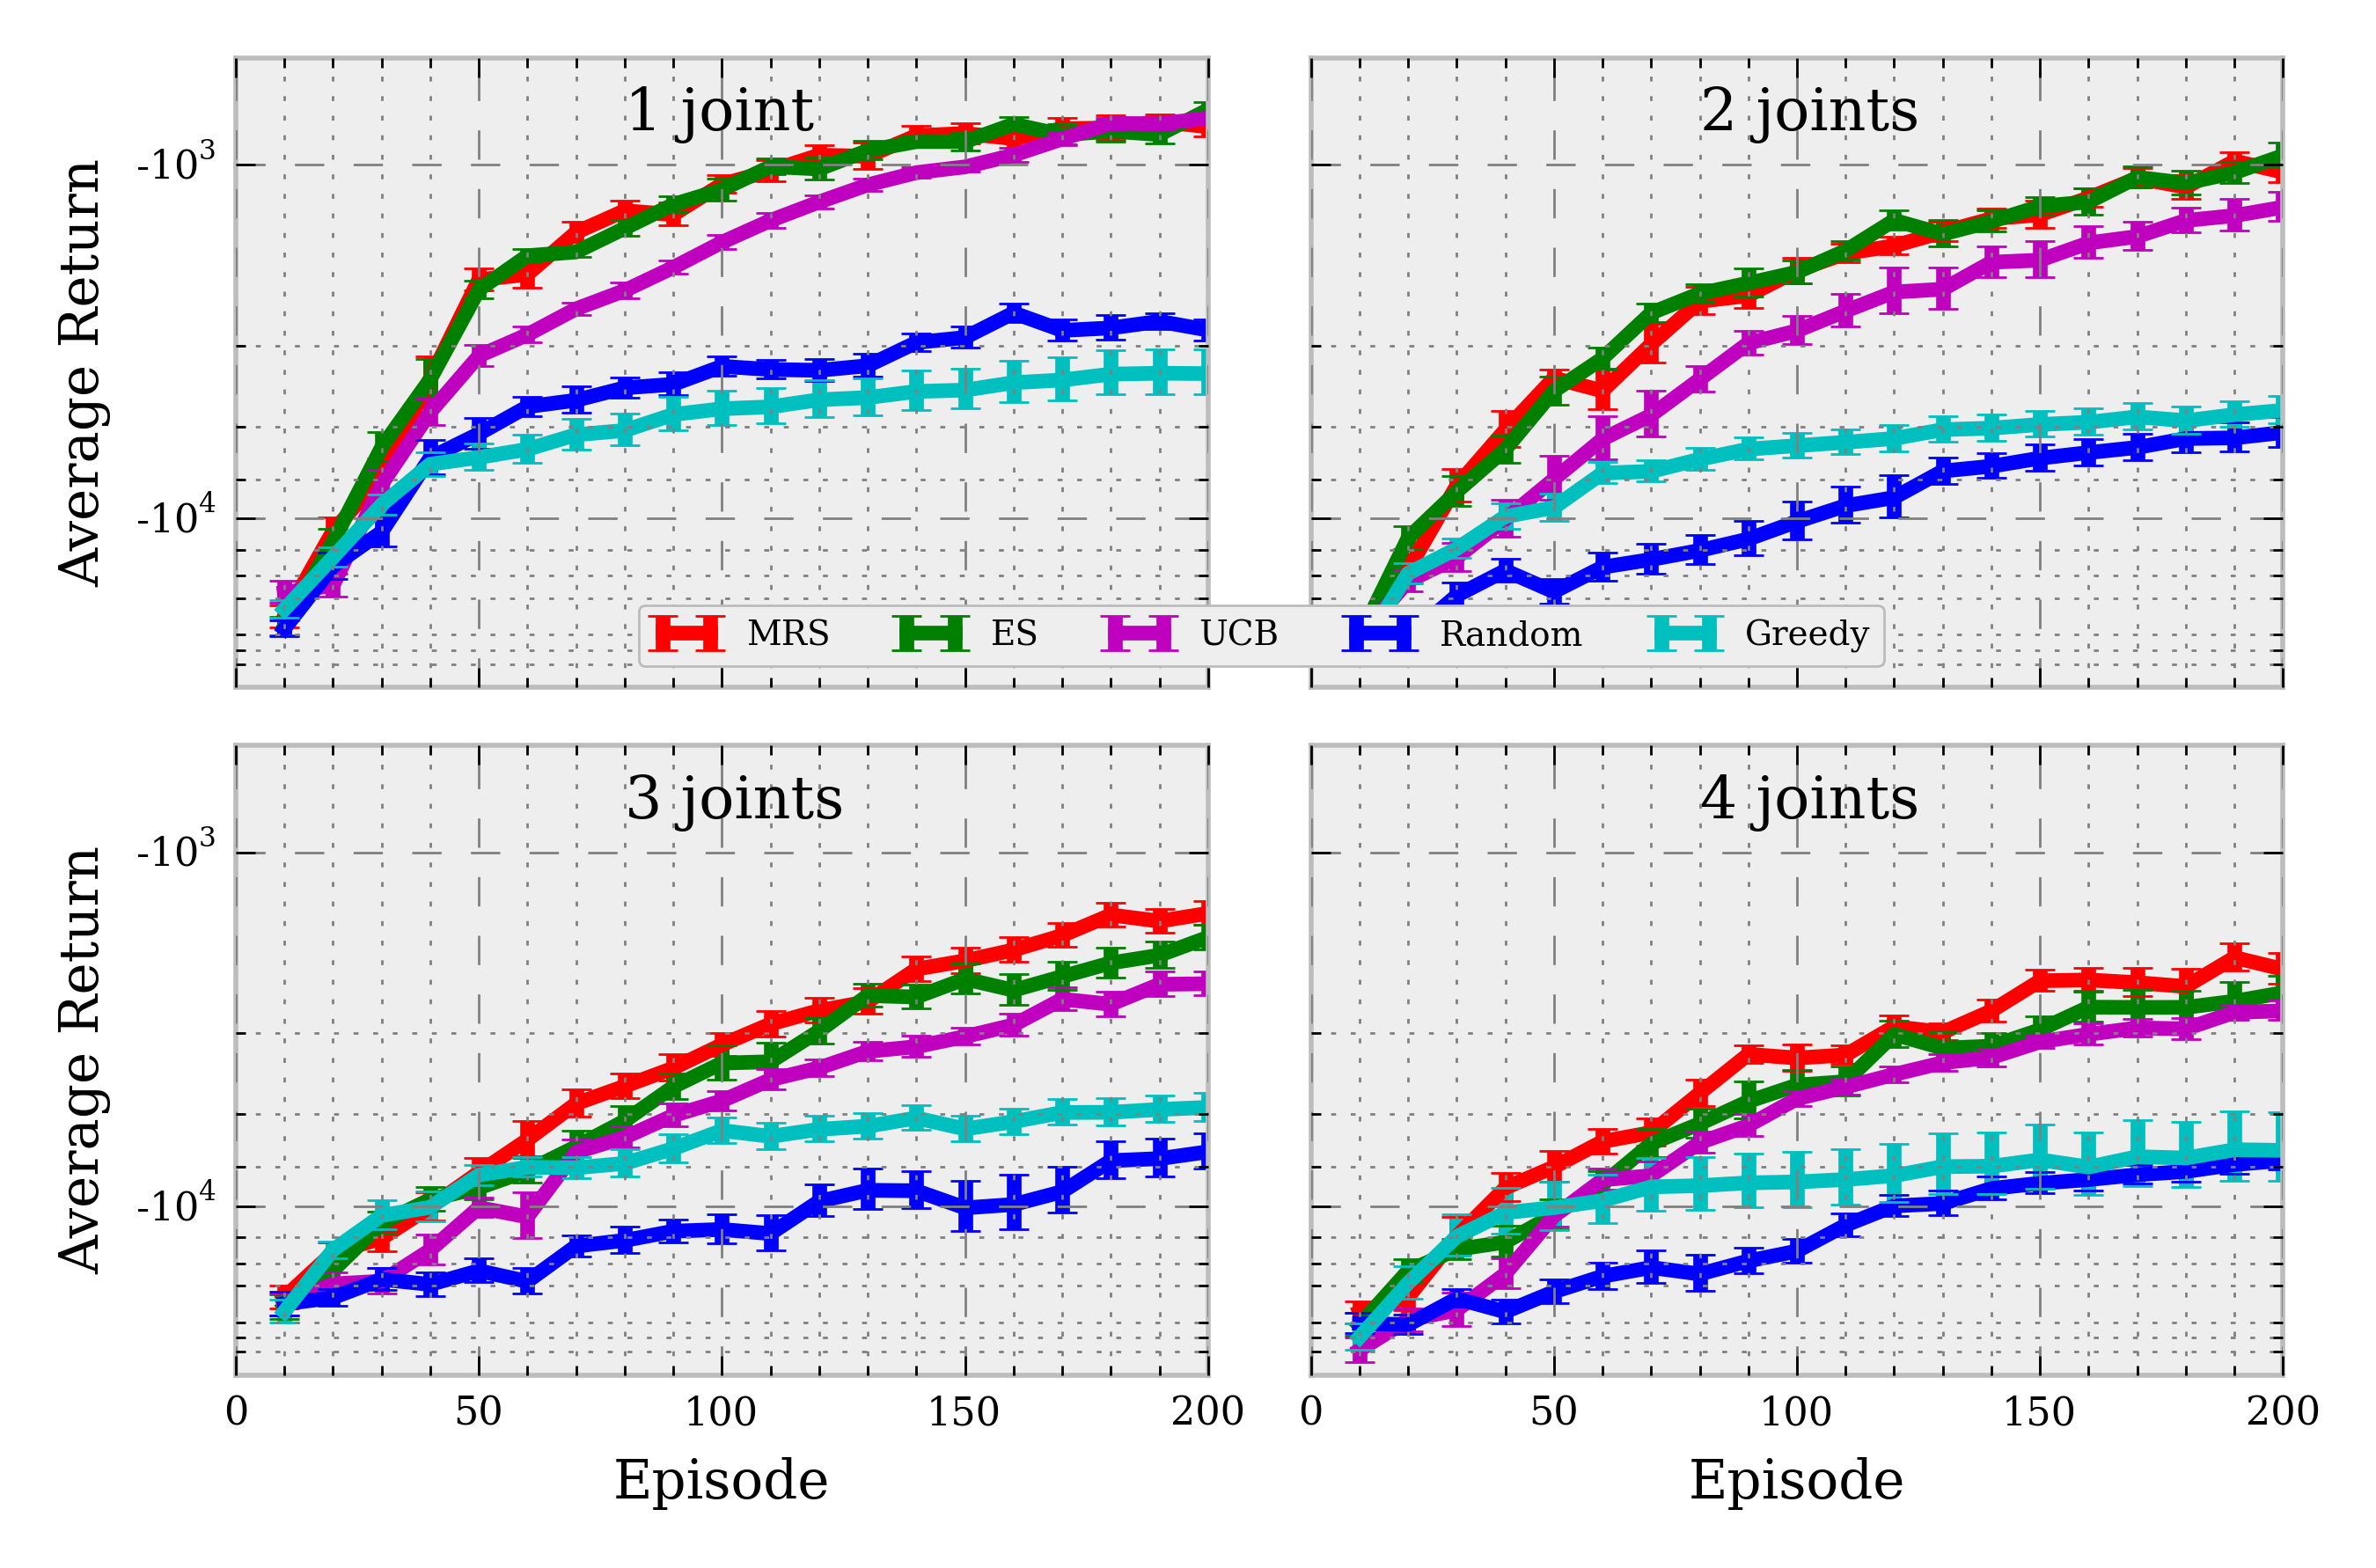
\includegraphics[width=.8\linewidth]{plots/learning_curve}\\
         Initial exploration covariance matrix matters (even with CMA-ES)
   \end{center}
\end{frame}

\begin{frame}{Outlook and Discussion}
  Open questions and future work:
  \begin{itemize}
    \item Correlated skill parameter dimensions: how to learn non-diagonal $\Omega \in \mathbb{R}^{m \times m}$ from small set of source tasks?
    \item Off-task learning: how to learn from $\skillparam_{\taskparam}$ with $J(\skillparam_{\taskparam},\taskparam) \ll J(\skillparam_{\taskparam}^*,\taskparam)$?
    \item Best way to handle discontinuities in mapping $\Theta$ (like fore- vs.\,backhand)?
    \item Learn $\Theta$ using (non-parametric) regression or (parametric) policy search?
    \pause
    \item Evaluation on humanoid robot AILA (simulated and real)
  \end{itemize}

  \begin{center}
    \includegraphics[width=.39\linewidth]{AILA}
  \end{center}
  \pause
  \begin{center}
   Thank you for your attention!
   Do you have questions, comments, or ideas?
   \end{center}

\end{frame}

\end{document}
